\section{Потоки}
Пусть у нас есть ориентированный граф. 
По этому графу течет некоторая \textit{жижа}.
Есть исток и есть сток, для каждого ребра известна пропусканая способность.

\begin{center}
    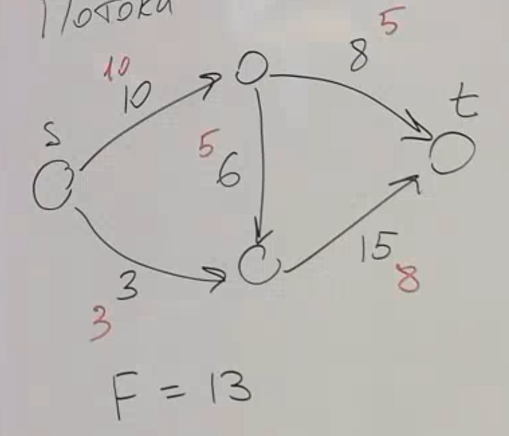
\includegraphics[scale=0.8]{img/flows_ex1.png}
\end{center}

Обозначим $C_{uv}$ --- пропусканая способность ребра, $f_{uv}$ --- величина потока.

$f_{uv} \geqslant 0$, $f_{uv} \leqslant c_{uv}$.

$\forall v \neq s, v \neq t ~:~ \sum\limits_u f_{uv} = \sum\limits_w f_{vw}$.

$F = \sum\limits_u f_{uv} - \sum\limits_w f_{vw}$

Решать такую задачу в такой формулировке не очень удобно. Удобнее мыслить в симеетричной формулировке, хочется избавиться от двух сумм. Давайте считать, что для каждого ребра есть фиктивный обратный поток.

\begin{center}
    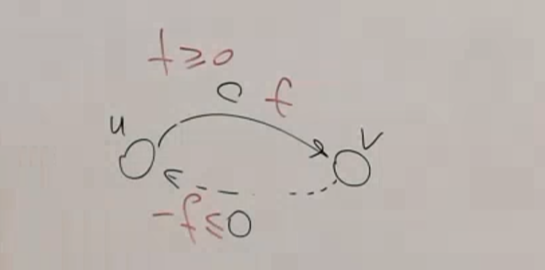
\includegraphics[scale=0.8]{img/flows_ex2.png}
\end{center}


$f_{vu} = - f_{uv}$, $c_{vu} = 0$, $f_{uv} \leqslant c_{uv}$

$\sum_u f_{vu} = 0$, $\forall v$ кроме s и t.

$F = \sum_u f_{su} = \sum_w f_{wt}$.

$\sum_v \sum_u f_{vu} = \sum f_{su} + \sum f_{tu}$.

На самом деле, не всегда можно просто так скаладывать потки $F = F_1 + F_2$. --- не всегда валидный поток (может переполниться ребро)

\begin{theorem} (Как бы утверждение)
    Любой поток можно декомпозировать на маленькие потоки
    \[F = F_1 + F_2 + \ldots + F_k\]

    $F_i$ -- путь $S \rightarrow t$ или цикл
\end{theorem}
\begin{proof}
    План: взять путь и вычесть его. Как найти какой-нибудь путь?

    \begin{enumerate}
        \item Пойдём из $S$
        \item Возьмём любое ребро по которому течёт жижа. 
        \item Рано или поздно либо дойдём до $t$, либо зациклимся.
    \end{enumerate}

    Хорошо, мы нашли путь. Давайте удалим его, в терминах потоков надо взять минимальную пропускную способность ребра и вычесть из всех ребер. 

    \begin{center}
        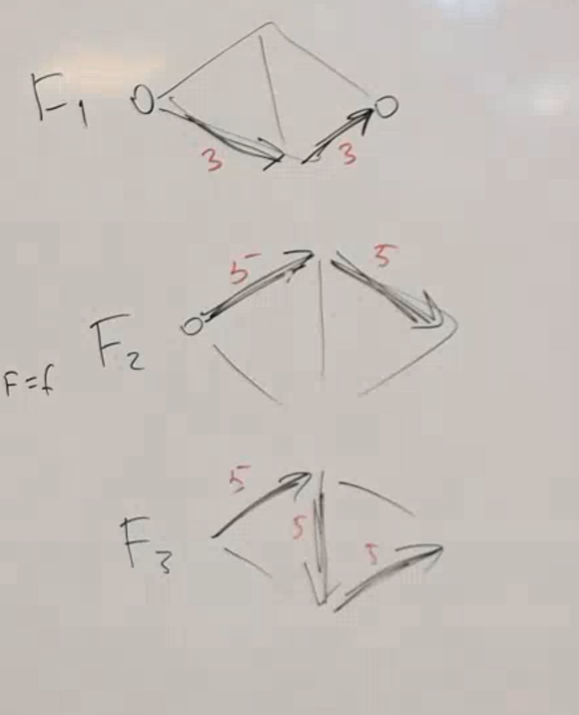
\includegraphics[scale=0.5]{img/flows_splitting.png}
    \end{center}

    Может ситуация, что из $S$ все рёбра нулевые, в $t$ все рёбра нулевые, а где-то в середине что-то происходит. 
    Это значит, что остались только циклы. Для их нахождения нужно взять любое ненулевое ребро и запускаться уже от него.

    Всего будет $O(m)$ путей и циклов, т.к. мы каждый раз обнулям хотя бы одно ребро.
\end{proof}

Вообще, мы хотим найти максимальный поток. Мы сперва возьмем пустое разбиение, а потом будем его постепенно дополнчть.

\begin{definition}
    Ребро называется насыщенным, если вся его пропуская задействована. 
\end{definition}

\begin{definition}
    Блокирующий поток --- такой поток, что любой путь содержит насыщенное этим потоком ребро. Иными словами, в данной сети не найдётся такого пути из истока в сток, вдоль которого можно беспрепятственно увеличить поток.
\end{definition}

\begin{definition}
    [Остаточная сеть]
    Пусть у нас был валидный поток. Для каждого ребра посчитаем $c_{uv}^\prime = c_{uv} - f_{uv} \geqslant 0$. Остаточная сеть --- подграф исходного, где на прямых ребрах написаны $c_{uv}$, а на обратных ребрах остаточная пропускная способность $c_{uv}^\prime$.  
    
    \begin{center}
        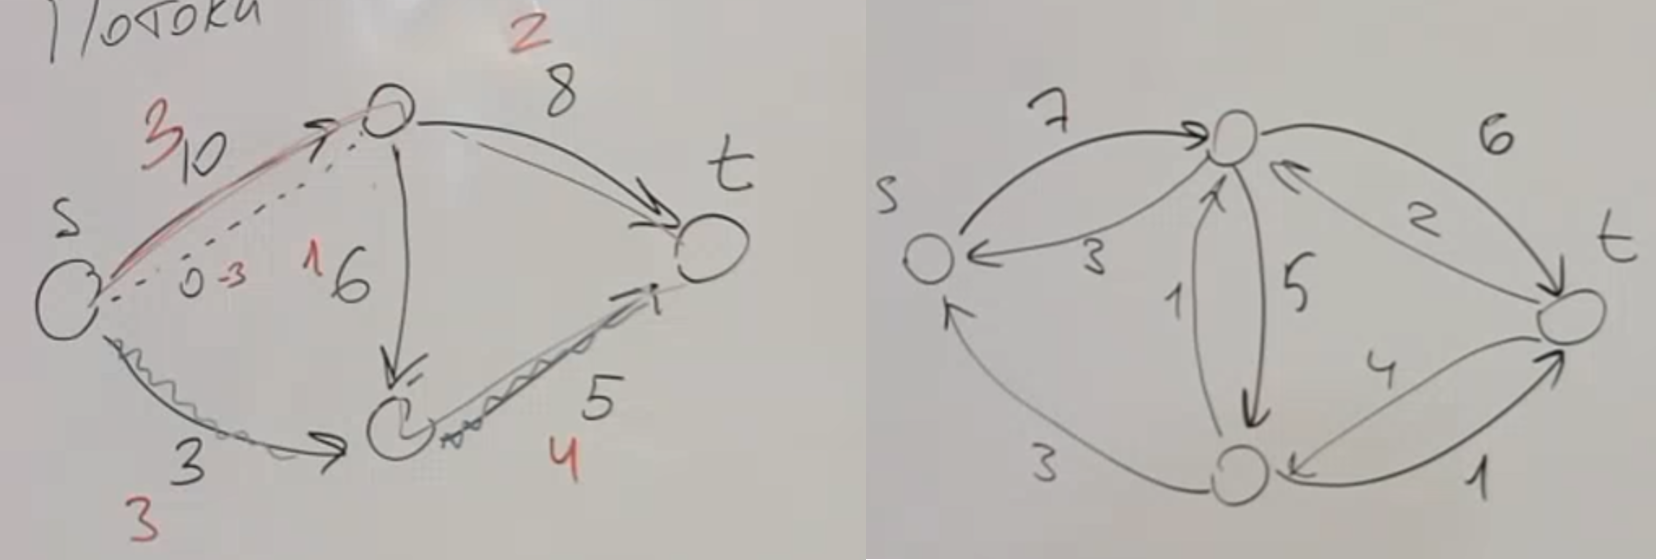
\includegraphics[scale=0.37]{img/flows_rest_network.png}
    \end{center}
\end{definition}

\subsubsection*{Идея алгоритма (схема Форда--Фалкерсона)}
\begin{itemize}
    \item Возьмём поток $F$, возтмём максимальный поток $F_{\max}$ и посмотрим на их разность $\Delta F = F_{\max} - F$
    \item
    $\Delta F$ --- поток в остаточной сети $C_{F}^\prime$
    $\Delta f_{uv} = f_{\max uv} - f_{uv} \leqslant C_{uv} - f_{uv} = C_{uv}^\prime$.
    \item Нет пути $S \to t$ в сети $C_F^\prime$ тогда и только тогда когда $F = F_{\max}$
\end{itemize}

\begin{lstlisting}[mathescape=true]
    int dfs(v, $\min \Delta$):
        if mark(v):
            return 0
        mark[v] = True
        for (uv): $C_{vu} - f_{uv} >0$
            $\Delta$ = dfs(u, $\min(\min\Delta, C_{uv} - f_{uv})$)
            if $\Delta > 0$:
                $f_{vu}$ += $\Delta$
                $f_{uv}$ -= $\Delta$
                return $\Delta$
        return 0
\end{lstlisting}

Время работы алгоритма --- $\mathcal{O}(F \cdot m)$.

\subsection{Разрезы}
\begin{problem}
Пусть есть граф. Мы хотим удалить некоторые ребра, чтобы не было пути из $S$ в $T$.
Определим $C = \sum c_{uv}$, для таких $u,v$, что нужно удалить ребро $uv$.

Надо найти $C_{\min}$.
\end{problem}

На самом деле это двойственная задача к поиску макимального потока.

Как искать минимальный разрез? Найдем максимальный поток, рассмотрим его дополняющую сеть. $\ldots$ ДОПИСАТЬ

\subsection{Алгоритм Эдмондса--Карпа}
Сделаем все то же самое, но dfs заменим на bfs.

Пусть $d[v]$ --- растояние (число ребер) от S до v в остаточной сети.

\begin{theorem}
    $d[v]$ не убывает, если выбирать кратчайшие лополняющие пути.
\end{theorem}
\begin{proof}
    Возьмем кратчайший путь $S \to T$. Ребра с минимальной дельтой на пути могли пропасть из остаточной сети. Какие могли добавться? Те, у которых были обратные ребра.

    Заметим, что $d[v]$ не убывает.

    Ребро может пропасть из дополняющей сети $d[u] = d[u] + 1$.\\
    Ребро может восстановавливаться в дополняющей сети $\p d[u]  = \p d [ v] + 1$.

    Таким образом $\p d [u] \geqslant d[u] + 2$.

    Поэтому ребро может быть добавлено и удалено не больше $\mathcal{O}(n)$ раз, а посколько ребер $m$, то всего таких запусков bfs может быть $\mathcal{O}(n m)$.
\end{proof}

Итого, наш алгоритм будет работать за $\mathcal{O}(n m^2)$. На самом деле, время работы асимптотически не больше, чем $\mathcal{O}(m \cdot F)$.

Анонс на дальше (что умеют люди):
\begin{enumerate}
    \item  $\mathcal{O}(nm)$ -- но стращно,такое смотреть небудем
    \item Плавно дойдём до $\mathcal{O}(nm \ln n)$
    \item $\mathcal{O}(nm\ln C)$
    \item $\mathcal{O}(n^3)$
\end{enumerate}

\begin{definition}
    [Масштабирование]
    Почему наш алгоритм работал долго? ПОтому что он искал плохие пути. Давайте запретим ему искать единичные пути. 
    Запустим ту же штуку, но на фазе $k$ заставим его брать пути длиной хотя бы $2^k$

    $k = \log C \ldots 0 $ искать пути $\Delta \geqslant 2^k $
\end{definition}
\begin{proof}
    $k+1 \to k $:

    $F_{\max} - F \leqslant 2^{k+1} \cdot m $

    Путей с $\Delta = 2^k\quad \leqslant 2m $

    Финальная асимптотика: $O(\ln C \cdot m^2 )$ -- слабополиномиальный алгоритм.
\end{proof}
\endinput